\documentclass[twocolumn,a4j]{jsarticle}
\setlength{\topmargin}{-20.4cm}
\setlength{\oddsidemargin}{-10.4mm}
\setlength{\evensidemargin}{-10.4mm}
\setlength{\textwidth}{18cm}
\setlength{\textheight}{26cm}

\usepackage[top=15truemm,bottom=25truemm,left=15truemm,right=15truemm]{geometry}
\usepackage[latin1]{inputenc}
\usepackage{amsmath}
\usepackage{amsfonts}
\usepackage{amssymb}
\usepackage[dvipdfmx]{graphicx}
\usepackage[dvipdfmx]{color}
\usepackage{listings}
\usepackage{listings,jvlisting}
\usepackage{geometry}
\usepackage{framed}
\usepackage{color}
\usepackage[dvipdfmx]{hyperref}
\usepackage{ascmac}
\usepackage{enumerate}
\usepackage{tabularx}
\usepackage{cancel}
\usepackage{scalefnt}

\renewcommand{\figurename}{Fig.}
\renewcommand{\tablename}{Table }

\lstset{
basicstyle={\ttfamily},
identifierstyle={\small},
commentstyle={\smallitshape},
keywordstyle={\small\bfseries},
ndkeywordstyle={\small},
stringstyle={\small\ttfamily},
frame={tb},
breaklines=true,
columns=[l]{fullflexible},
xrightmargin=0zw,
xleftmargin=3zw,
numberstyle={\scriptsize},
stepnumber=1,
numbersep=1zw,
lineskip=-0.5ex
}

\makeatletter
\def\@maketitle
{
\begin{center}
{\LARGE \@title \par}
\end{center}
\begin{flushright}
{\large 報告書 NO.06 - 2-1\quad\@date\quad\@author}
\end{flushright}
\par\vskip 1.5em
}
\makeatother

\setcounter{tocdepth}{3}

\author{来代 勝胤}
\title{令和3年度 10月 第3週 報告書}
\date{2021/10/21}

\begin{document}
\columnseprule=0.1mm

\maketitle
\section*{報告内容}
\begin{enumerate}[1.]
    \item 進捗状況
    \item FFTによる周波数特性の比較
    \item 校正実験装置のフレーム組立
\end{enumerate}
\section{進捗状況}
今週は、実験データを、
(1) 測定前 (2) 測定中 の2つの部分に分けてFFTを行い、
周波数特定について比較を行った。
また、ひずみゲージの実験装置に用いるフレームの組立を行った。

\section{FFTによる周波数特性の比較}
周波数解析を行うにあたり、解析範囲について以下のFig.1に示す。
回流水槽の水流発生時刻については、移動平均(n=11)を用いて特定した時刻を用いている。\\
※ 開始時刻 [s] = 移動平均(n=11)の開始時刻 [s] + 5 [s]\\

\subsection{FFTに利用する範囲の設定}
周波数解析に利用した範囲は、水流発生時刻を基準として、後部を Range 1 (作用力測定中)、
前部を Range 2 (水流発生前・タイヤモデルのみ回転) として設定している。
なお、水流開始時刻から Range 1 は60秒間、Range 2 は30秒間のデータを除いて使用している。
\begin{figure}[htbp]
    \footnotesize
    \begin{center}
        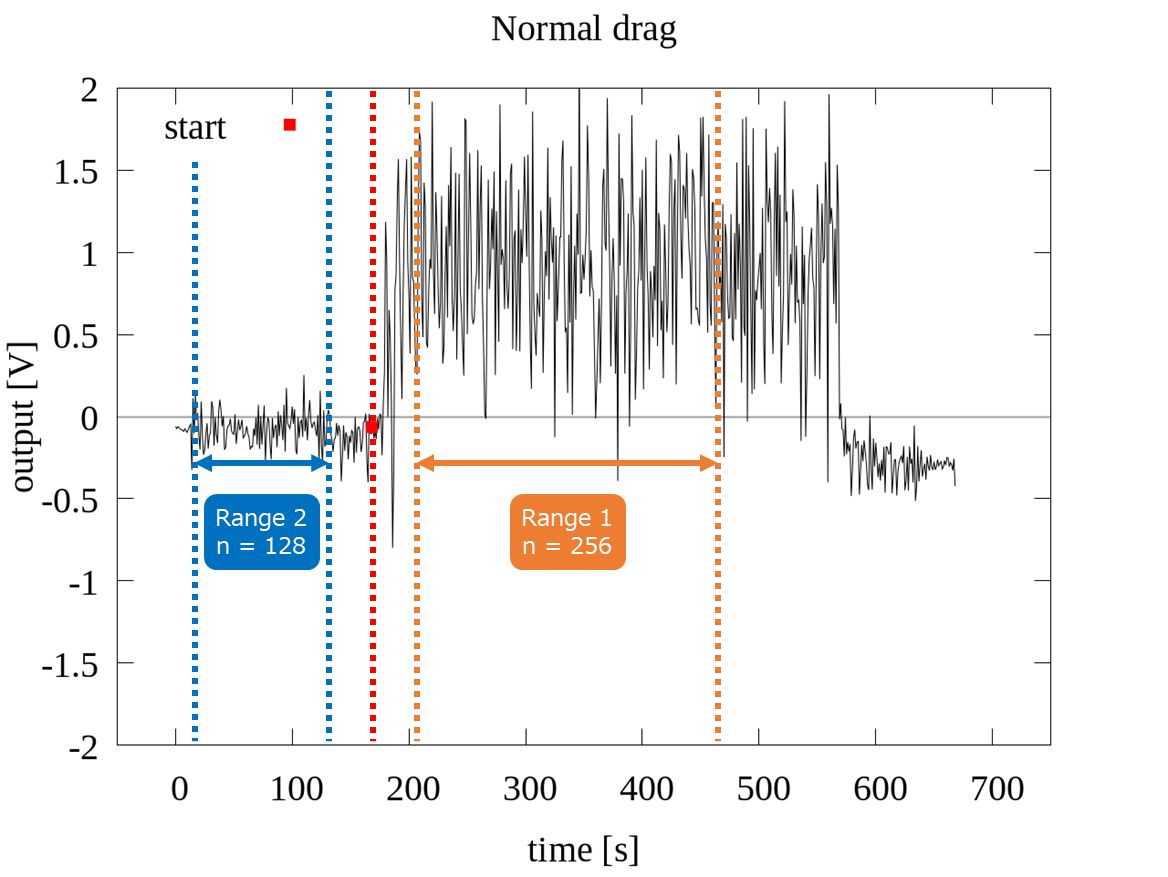
\includegraphics[width=90mm]{../images/image_1.png}
        \caption{Range of FFT}
    \end{center}
\end{figure}

\subsection{解析結果}
FFTによる解析結果は以下 Fig.2 ~ Fig.4のようになった。
なお、今回のFFT解析には、2021年8月6日(金) 実施の実験データを使用している。\\
\subsubsection{Normal Drag}
\begin{figure}[htbp]
    \footnotesize
    \begin{center}
        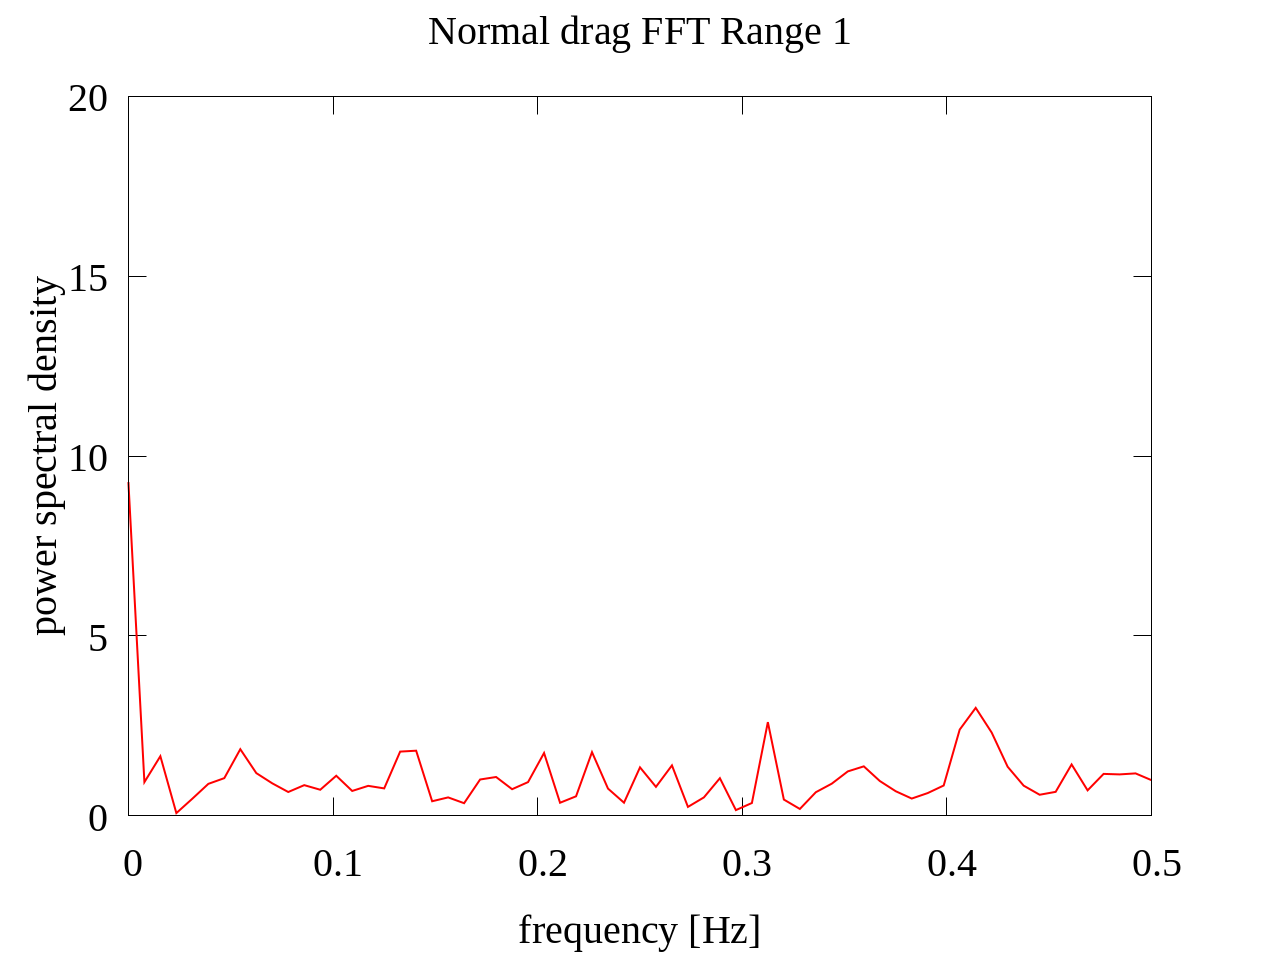
\includegraphics[width=85mm]{../images/Normal_drag_06.png}
        \caption{Normal's drag Range1 result}
        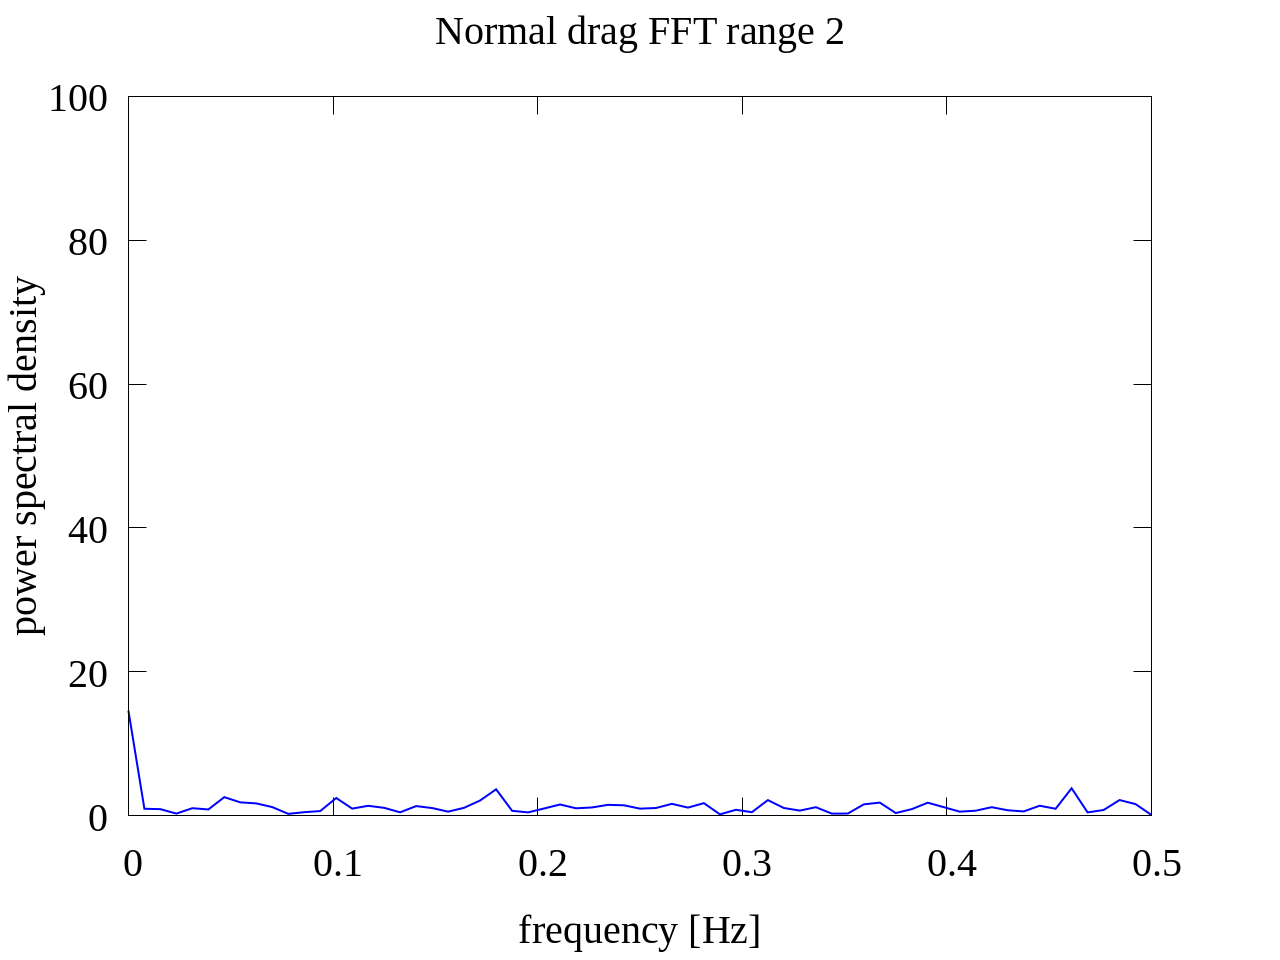
\includegraphics[width=85mm]{../images/Normal_drag_07.png}
        \caption{Normal's drag Range2 result}
    \end{center}
\end{figure}
\newpage
\subsubsection{Normal Lift}
\begin{figure}[htbp]
    \footnotesize
    \begin{center}
        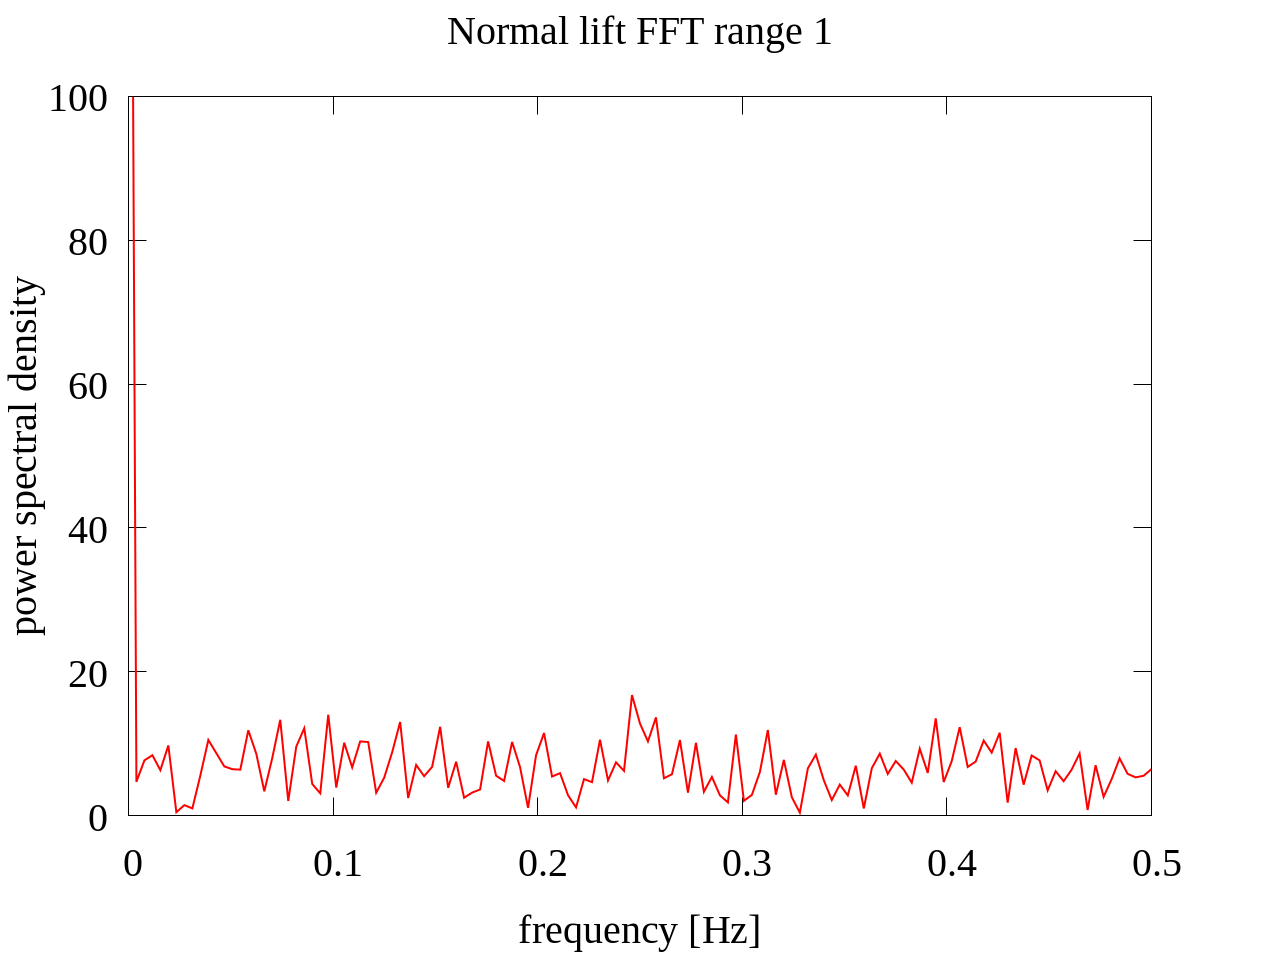
\includegraphics[width=85mm]{../images/Normal_lift_06.png}
        \caption{Normal's lift Range1 result}
        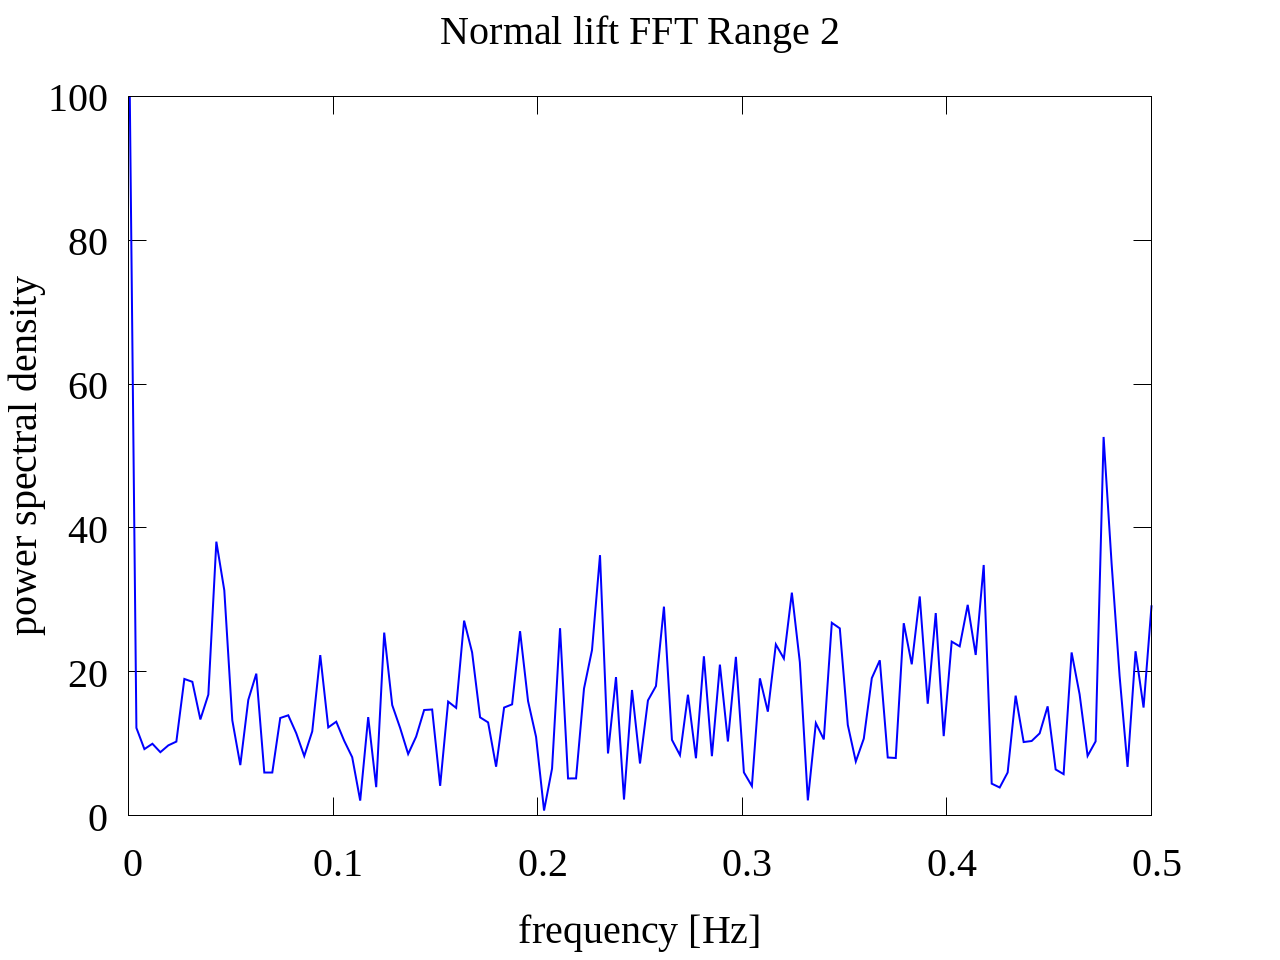
\includegraphics[width=85mm]{../images/Normal_lift_07.png}
        \caption{Normal's lift Range2 result}
        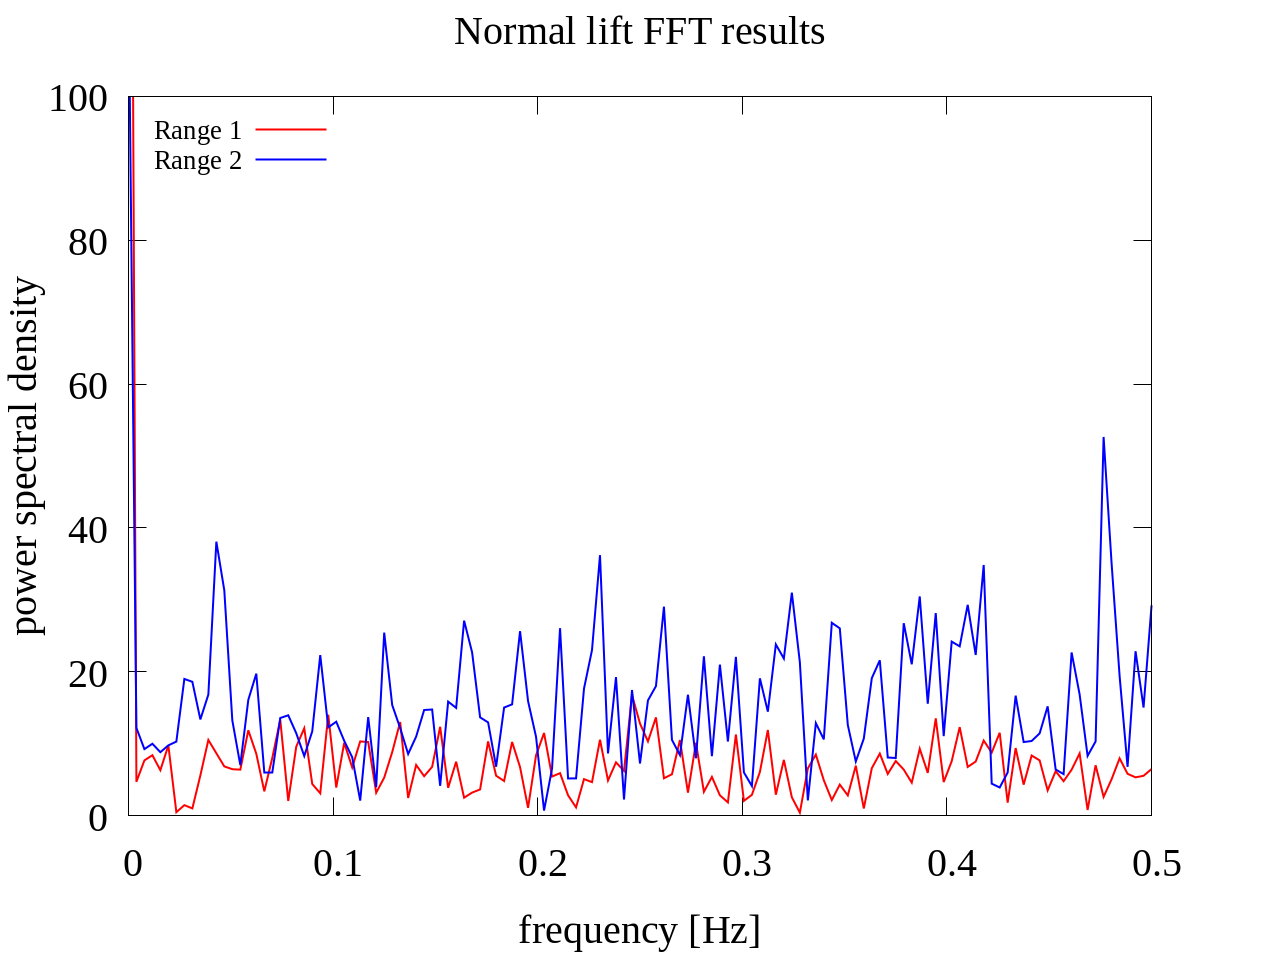
\includegraphics[width=85mm]{../images/Normal_lift_08.png}
        \caption{Normal'lift result}
    \end{center}
\end{figure}
\newpage
\section{校正実験装置のフレーム組立}

\end{document}